\documentclass[12pt, a4paper]{paper}
\usepackage{amsmath}
\usepackage{graphicx}
\usepackage{subcaption}
\usepackage{caption}
\usepackage{cite}
\usepackage{apacite}
%\usepackage[a4paper,top=xcm,bottom=xcm,left=xcm,right=xcm]{geometry}
 

\begin{document}

\author{Montese Sara, Pasquini Gioele, Terrenzi Riccardo}

\title{Memristor oscillator on Matlab}
\maketitle
\begin{figure}[h]
\centering
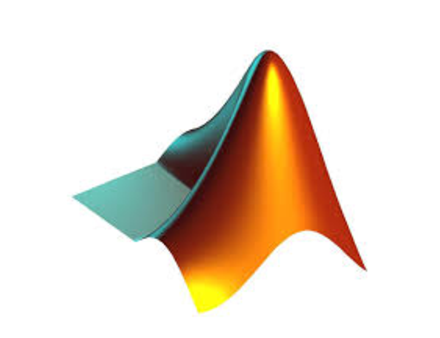
\includegraphics[width=0.6\textwidth]{matsimbol_1.eps}
\end{figure}
\newpage
\tableofcontents
\newpage

\section{Introduction}
\subsection{What's a memristor?}
\begin{figure}[h]
\centering
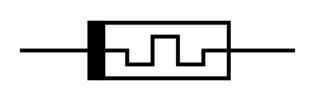
\includegraphics[width=0.8\textwidth]{mem2.eps}
\end{figure}
A memristor, or memory resistor, is described as one of the basic elements (resistor, capacitor, inductor) of electronic circuits, because it can’t be replaced by any combination of these elements.

\begin{figure}[h]
\centering
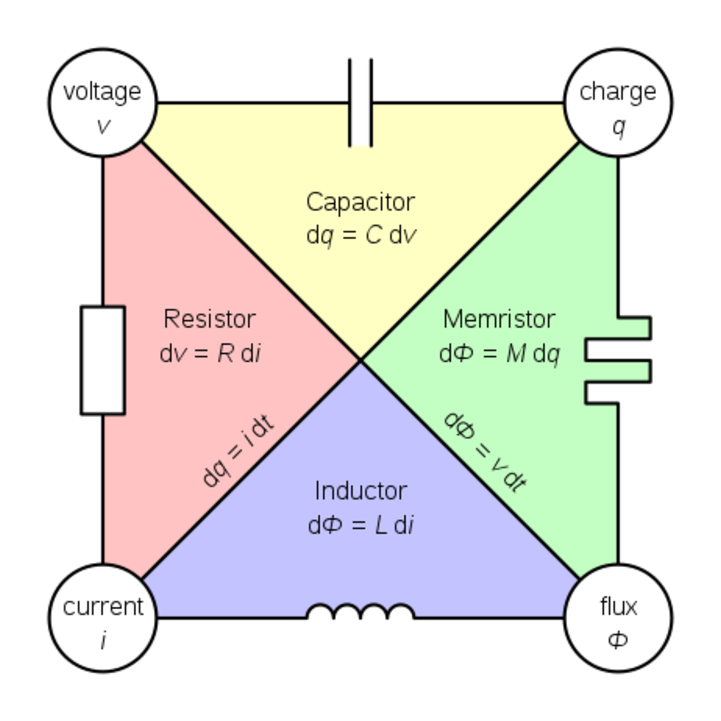
\includegraphics[width=0.8\textwidth]{componenti_fondamentali_1.eps}
\end{figure}

This element can change its resistivity according to the voltage, but even after disconnection it remembers resistivity for unlimited time. It can work like analog memory or a resistive switch, which can have an infinite number of states.
Memristor is a passive two-terminal electronic device described by the nonlinear
constitutive relation

                     $v=M(q)i$ or $i=W(\phi)v$

 between the device terminal voltage v and 
terminale current i.

The memeristor constitutive relation is represented by the memristance and the
memductance, defined by these equations: 

$M(q) = \frac{d\phi(q)}{dq} $ and

$ W(\phi)=\frac{dq(\phi)}{d\phi}$

In particular, we note that a memristor is passive if, and only if, its 
memristance is non-negative:

$M(q)=\frac{d\phi(q)}{dq}\geq 0$

We assume that the memristor is characterized by the “monotone-increasing" and
“piecewise-linear" nonlinearity: 

$\phi(q)=bq+0.5(a-b)(|q+1|-|q-1|)$ and 

$q(\phi)=d\phi+0.5(c-d)(|\phi+1|-|\phi-1|)$

 Consequently, the memristance and the memductance are defined by: 
 
\begin{equation}
M(q)=\frac{d\phi(q)}{dq}=
\begin{cases}
a, |q|<1
\\
b, |q|>1
\end{cases}
\end{equation}

\begin{equation}
W(\phi)=\frac{dq(\phi)}{d\phi}=
\begin{cases}
c, |\phi|<1
\\
d, |\phi|>1
\end{cases}
\end{equation}

\subsection{History}

Leon Chua postulated the idea of memristor in 1971, but the first real memristor
was build only in 2008 by R. Stanley Williams from the Hewlett-Packard Company.
The device instantly generated interest all over the world for its potential
applications, for example in non-volatible memories, in next-generation computers,
but also in cryptography.

\subsection{Our project}

The main topic of our project is the Matlab implementation of all the plots we
can see in the paper \cite{itoh2008memristor}.
We studied the functions of various types of chaotic oscillators and figured out how
to represent the trajectories that these oscillators generate on a plot.
So, mainly, we implemented these functions on Matlab, solved differential 
equations numerically using ODE45 and drew plots.

But we'll see the details of our work in the next pages.

\newpage
\section{Plots and equations}

\subsection{Fig.10}
Fourth-order canonical memristor oscillator:
\subsubsection{Equations}
\begin{equation}
\begin{cases}
\frac{dx}{dt}=\alpha(y-W(\omega)x) 
\\
\frac{dy}{dt}=z-x
\\
\frac{dz}{dt}=-y\beta+z\gamma
\\
\frac{d\omega}{dt}=x
\\
\end{cases}
\end{equation}

\textbf{Variables}: $x=v_1, y=i_3, z=v_2, \omega=\phi, \alpha=\frac{1}{C_1},
\beta=\frac{1}{C_2}, \gamma=\frac{G}{C_2}, L=1$.

\textbf{Parameters}: $\alpha =4, \beta =1, \gamma =0.65, a=0.2, b=10$.

You can find the following equations:

$q(\omega)$ and $W(\omega)$, in \textit{page 5}.

\begin{figure}[h]
\centering
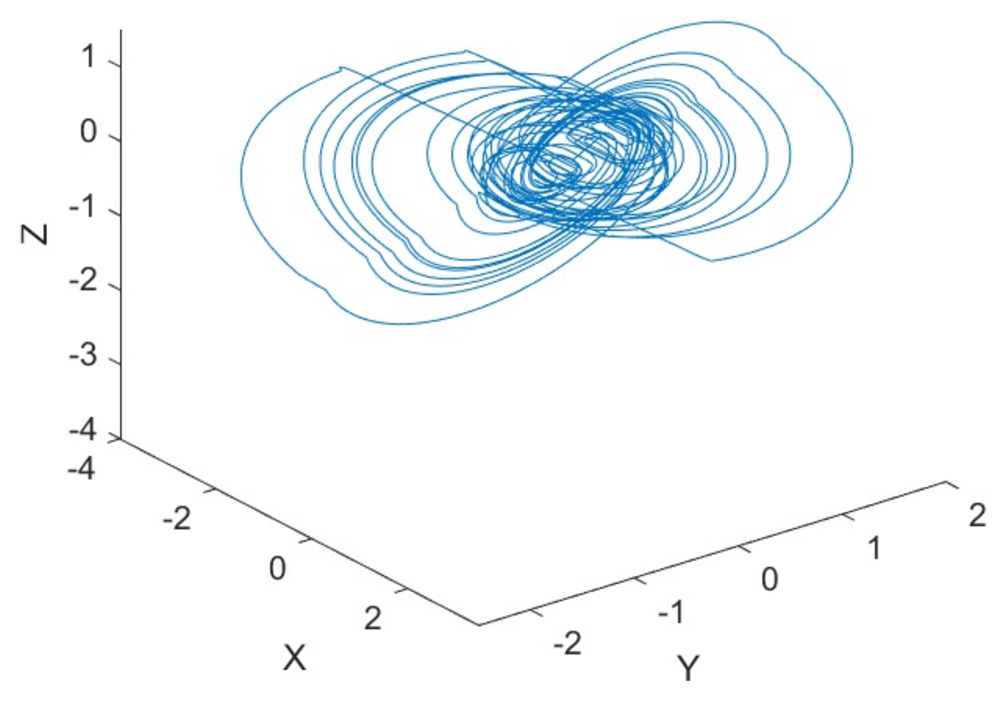
\includegraphics[width=0.4\textwidth]{Fig_10_1.eps}
\caption{This graphic shows the evolution over time of Z, X and Y}
\end{figure}

\begin{figure}[h]
\centering
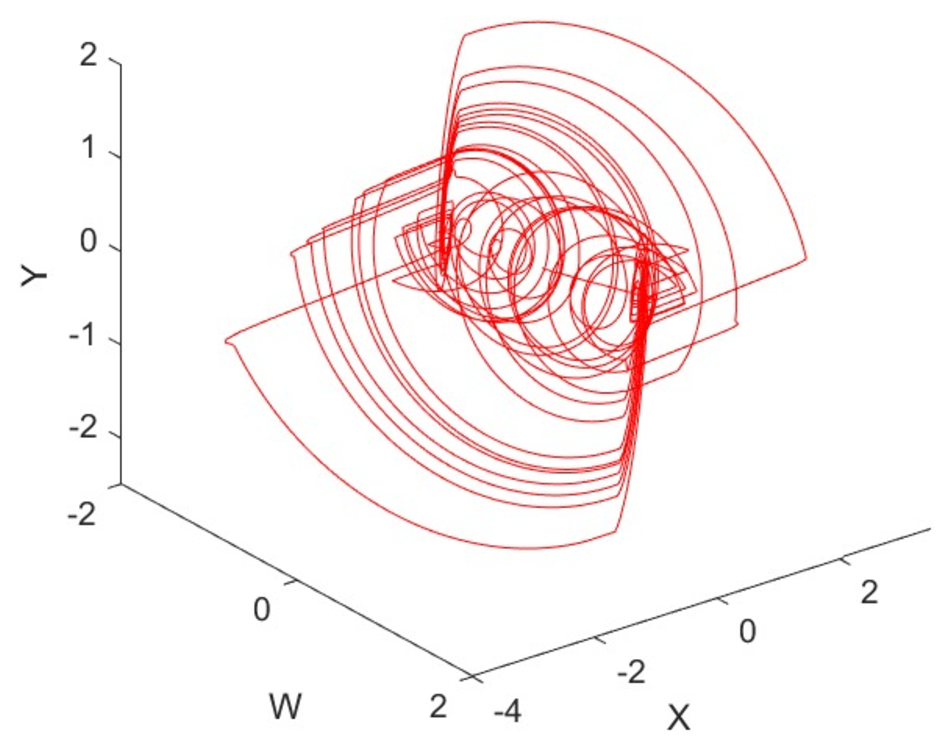
\includegraphics[width=0.4\textwidth]{Fig_10_2.eps}
\caption{This graphic shows the evolution over time of W, X and Y}
\end{figure}

\newpage
\subsection{Fig.12}
Fourth-order canonical memristor oscillator:
\subsubsection{Equations}
\begin{equation}
\begin{cases}
\frac{dx}{dt}=\alpha(y-W(\omega)x)
\\
\frac{dy}{dt}=-\xi(x+z)
\\
\frac{dz}{dt}=y\beta
\\
\frac{d\omega}{dt}=x
\\
\end{cases}
\end{equation}

\textbf{Variables}: $x=v_1, y=i_3, z=-v_2, \omega=\phi, \alpha=\frac{1}{C_1},
\beta=\frac{1}{C_2}, \xi=\frac{1}{L}$.

\textbf{Parameters}: $\alpha =4.2, \beta =-20, \xi =-1, a=-2, b=9$.

you can find the following equations:

$q(\omega)$ and $W(\omega)$, in \textit{page 5}.

\begin{figure}[h]
\centering
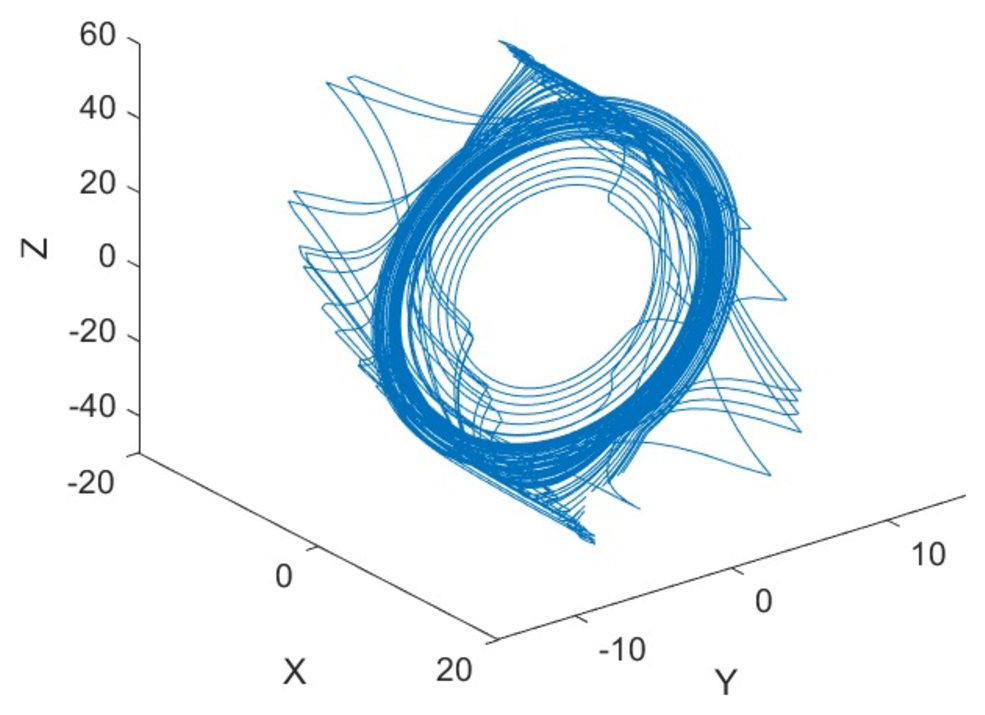
\includegraphics[width=0.4\textwidth]{Fig_12_1.eps}
\caption{This graphic shows the evolution over time of Z, X and Y}
\end{figure}

\begin{figure}[h]
\centering
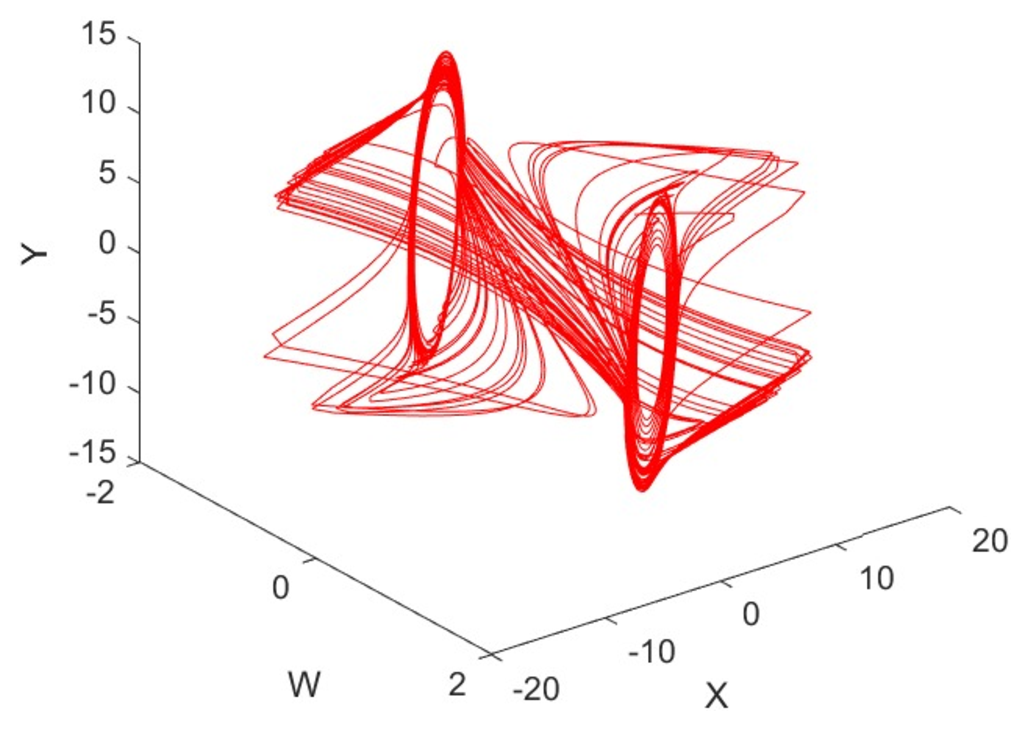
\includegraphics[width=0.4\textwidth]{Fig_12_2.eps}
\caption{This graphic shows the evolution over time of W, X and Y}
\end{figure}


\newpage
\subsection{Fig.17}
Third-order canonical memristor oscillator:
\subsubsection{Equations}
\begin{equation}
\begin{cases}
\frac{dx}{dt}=\alpha(y-W(z)x)
\\
\frac{dy}{dt}=-\xi x+\beta y
\\
\frac{dz}{dt}=x
\\
\end{cases}
\end{equation}

\textbf{Variables}: $x=v_1, y=i_3, z=\phi, \alpha=\frac{1}{C_1},
\beta=\frac{R}{L}, \xi=\frac{1}{L}$.

\textbf{Parameters}: $\alpha =1, \beta =0.1, \xi =1, a=0.02, b=2$.

you can find the following equations:

$q(z)$ and $W(z)$, in \textit{page 5}.

\begin{figure}[h]
\centering
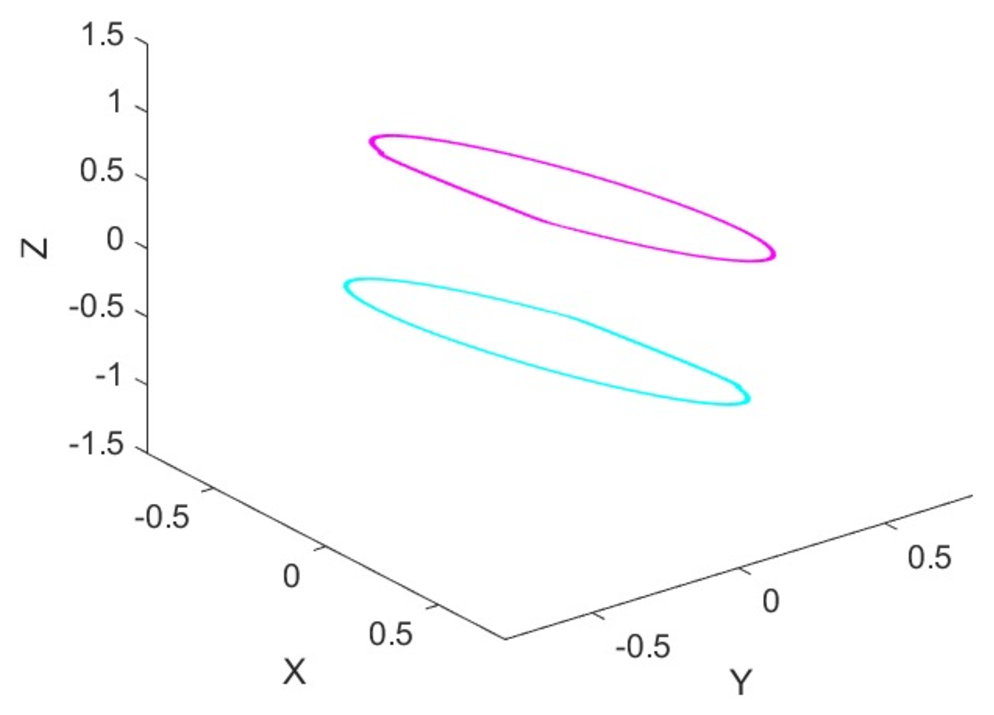
\includegraphics[width=1\textwidth]{Fig_17.eps}
\caption{This graphic shows the evolution over time of Z, X and Y with two different sets of parameters}
\end{figure}

\newpage
\subsection{Fig.23}
Second-order canonical memristor oscillator:
\subsubsection{Equations}
\begin{equation}
\begin{cases}
\frac{dx}{dt}=\alpha(\beta-W(y)x)
\\
\frac{dy}{dt}=x
\\
\end{cases}
\end{equation}

\textbf{Variables}: $x=v_1, y=\phi, \alpha=\frac{1}{C_1},
\beta=G$.

\textbf{Parameters}: $\alpha =1, \beta =0.03, a=0.01, b=0.03$.

you can find the following equations: 

$q(y)$ and $W(y)$, in \textit{page 5}.

\begin{figure}[h]
\centering
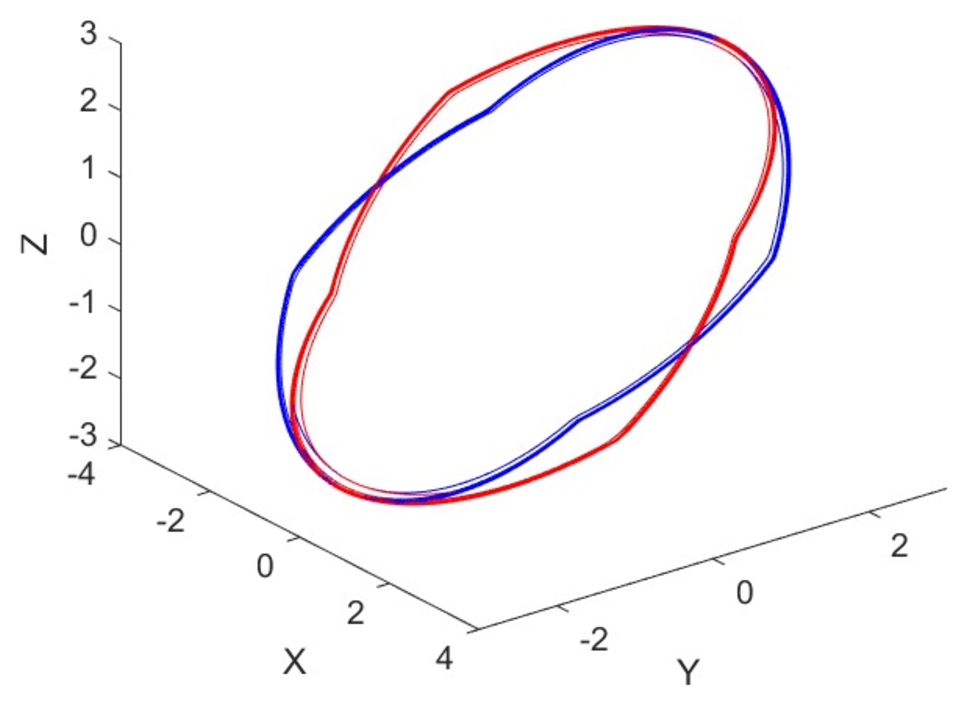
\includegraphics[width=1\textwidth]{Fig_23.eps}
\caption{This graphic shows the evolution over time of Z, X and Y with two different sets of parameters}
\end{figure}

\newpage
\subsection{Fig.26}
Fourth-order canonical memristor oscillator:
\subsubsection{Equations}
\begin{equation}
\begin{cases}
\frac{dx}{dt}=\alpha(y-x+x\xi-W(\omega)x)
\\
\frac{dy}{dt}=x-y+z
\\
\frac{dz}{dt}=-y\beta-z\gamma
\\
\frac{d\omega}{dt}=x
\\
\end{cases}
\end{equation}

\textbf{Variables}: $x=v_1, z=-i, y=v_2, \omega=\phi, \alpha=\frac{1}{C_1},
\beta=\frac{1}{L}, \gamma=\frac{r}{L},$ 

$\xi=G, C_2=1, R=1$.

\textbf{Parameters}: $\alpha =10, \beta =13, \gamma =0.35, \xi=1.5, a=0.3, b=0.8$.

you can find the following equations:

$q(\omega)$ and $W(\omega)$, in \textit{page 5}.
\begin{figure}[h]
\centering
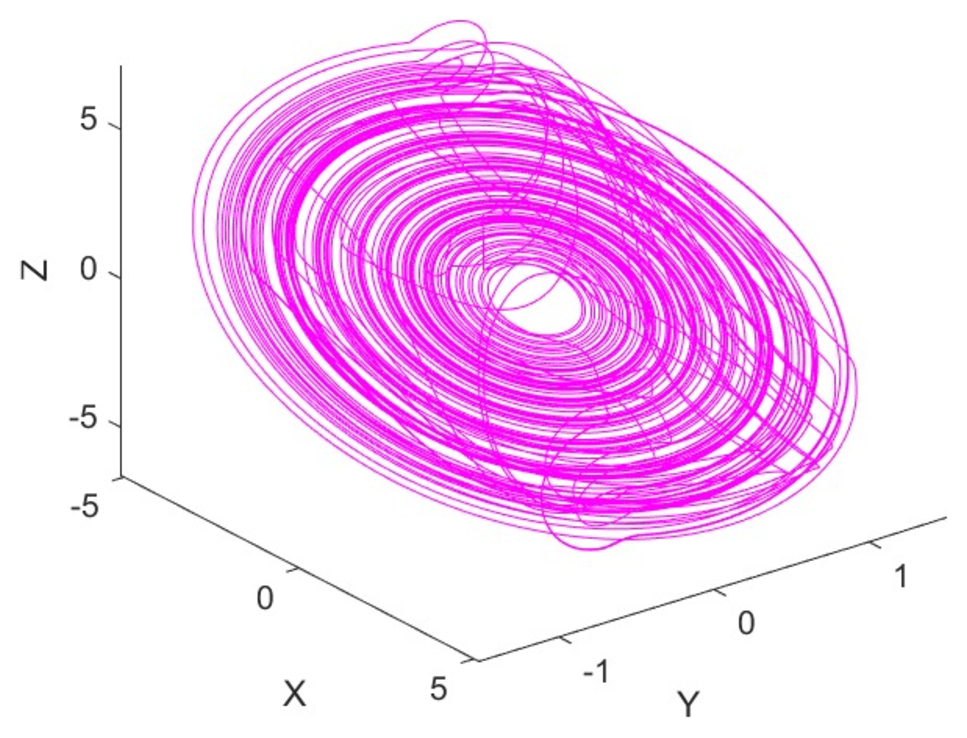
\includegraphics[width=0.4\textwidth]{Fig_26_1.eps}
\caption{This graphic shows the evolution over time of Z, X and Y}
\end{figure}

\begin{figure}[h]
\centering
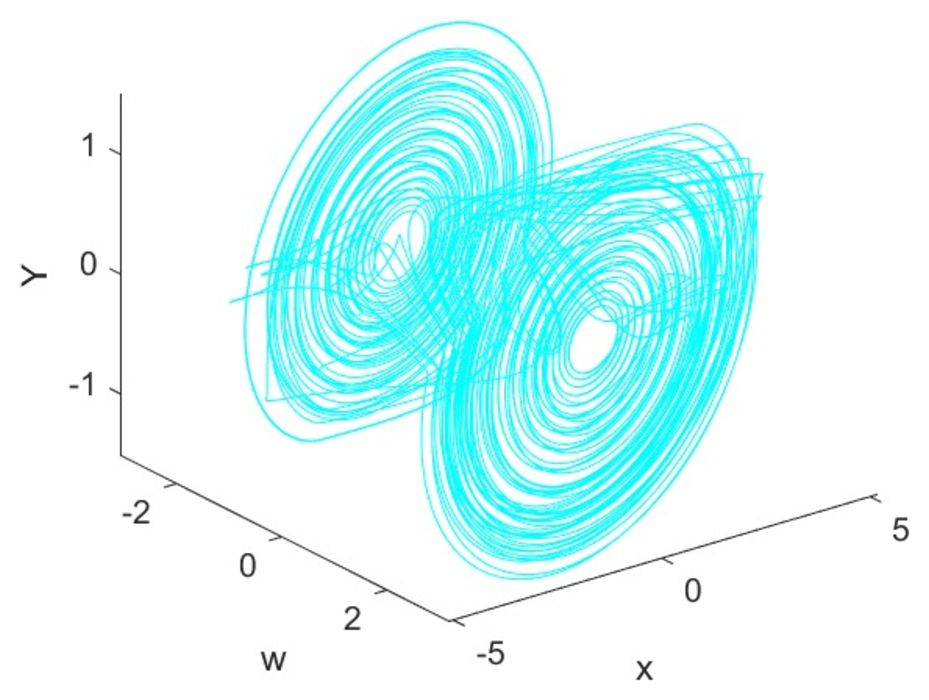
\includegraphics[width=0.4\textwidth]{26_2.eps}
\caption{This graphic shows the evolution over time of W, X and Y}
\end{figure}


\newpage
\subsection{Fig.29}
Third-order canonical memristor oscillator:
\subsubsection{Equations}
\begin{equation}
\begin{cases}
\frac{dx}{dt}=\alpha(y-W(z)x+\gamma x)
\\
\frac{dy}{dt}=\beta x
\\
\frac{dz}{dt}=x
\\
\end{cases}
\end{equation}

\textbf{Variables}: $x=v, y=i, z=\phi, \alpha=\frac{1}{C},
\beta=\frac{1}{L}, \gamma=G$.

\textbf{Parameters}: $\alpha =2, \beta =1, \gamma =0.3, a=0.1, b=0.5$.

you can find the following equations:

$q(z)$ and $W(z)$, in \textit{page 5}.

\begin{figure}[h]
\centering
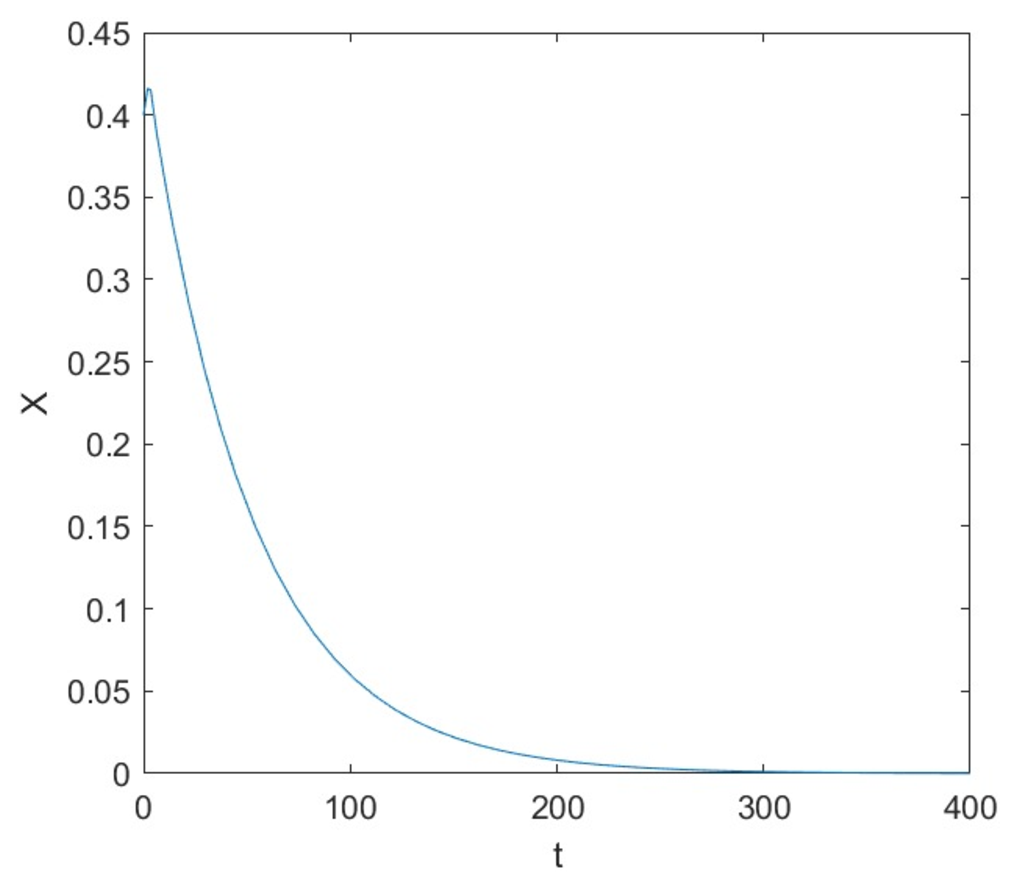
\includegraphics[width=0.8\textwidth]{Fig_29.eps}
\caption{This graphic shows the evolution over time of X}
\end{figure}

\newpage
\subsection{Fig.32}
Second-order canonical memristor oscillator:
\subsubsection{Equations}
\begin{equation}
\begin{cases}
y=(\gamma-W(z))x
\\
\frac{dy}{dt}=\beta x
\\
\frac{dz}{dt}=x
\\
\end{cases}
\end{equation}

\textbf{Variables}: $x=v, y=i, z=\phi, 
\beta=\frac{1}{L}, \gamma=G$.

\textbf{Parameters}: $\beta =1, \gamma =1, c=1$.

you can find the following equations:

$q(z)$ and $W(z)$, in \textit{page 5}.

\begin{figure}[h]
\centering
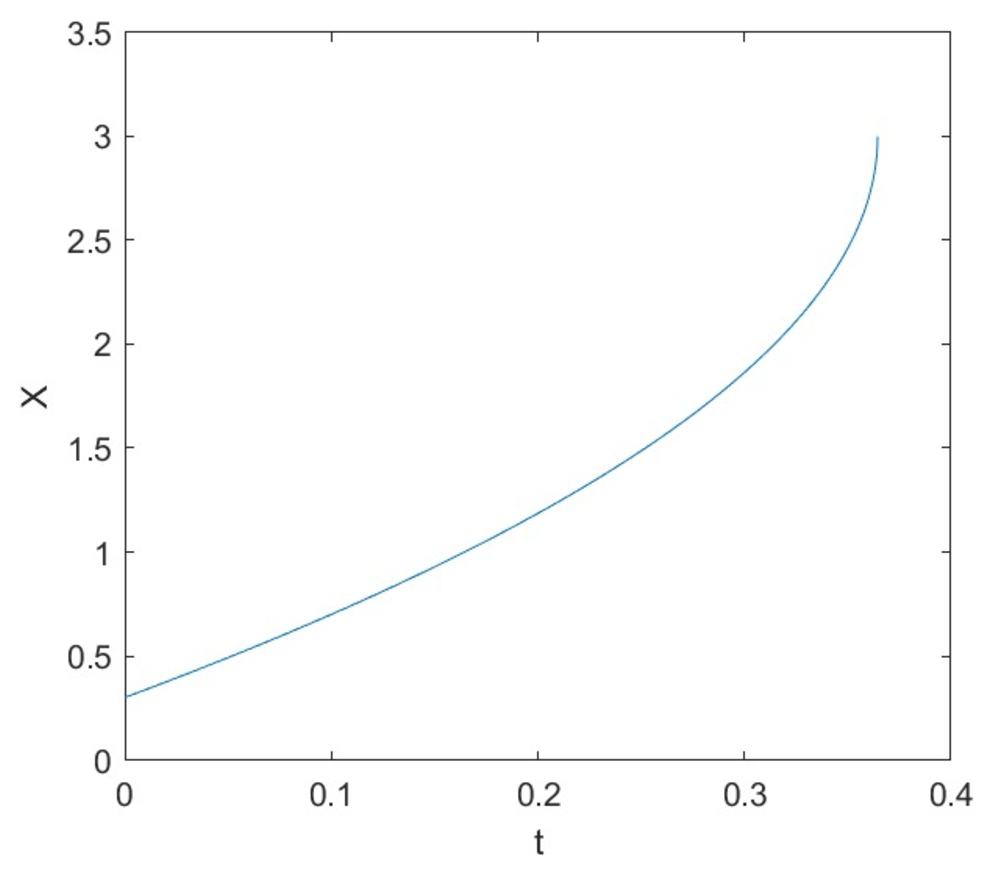
\includegraphics[width=0.8\textwidth]{Fig_32.eps}
\caption{This graphic shows the evolution over time of X}
\end{figure}

\newpage
\subsection{Fig.36}
First-order canonical memristor oscillator:
\subsubsection{Equations}
\begin{equation}
\begin{cases}
\frac{dx}{dt}=\frac{e}{W(x)-\beta}
\end{cases}
\end{equation}

\textbf{Variables}: $x=\phi, e=J, \beta=G$.

\textbf{Parameters}: $\beta =0.3, e=1$.

you can find the following equations:

$q(x)$ and $W(x)$, in \textit{page 5}.



\begin{figure}[h]
\centering
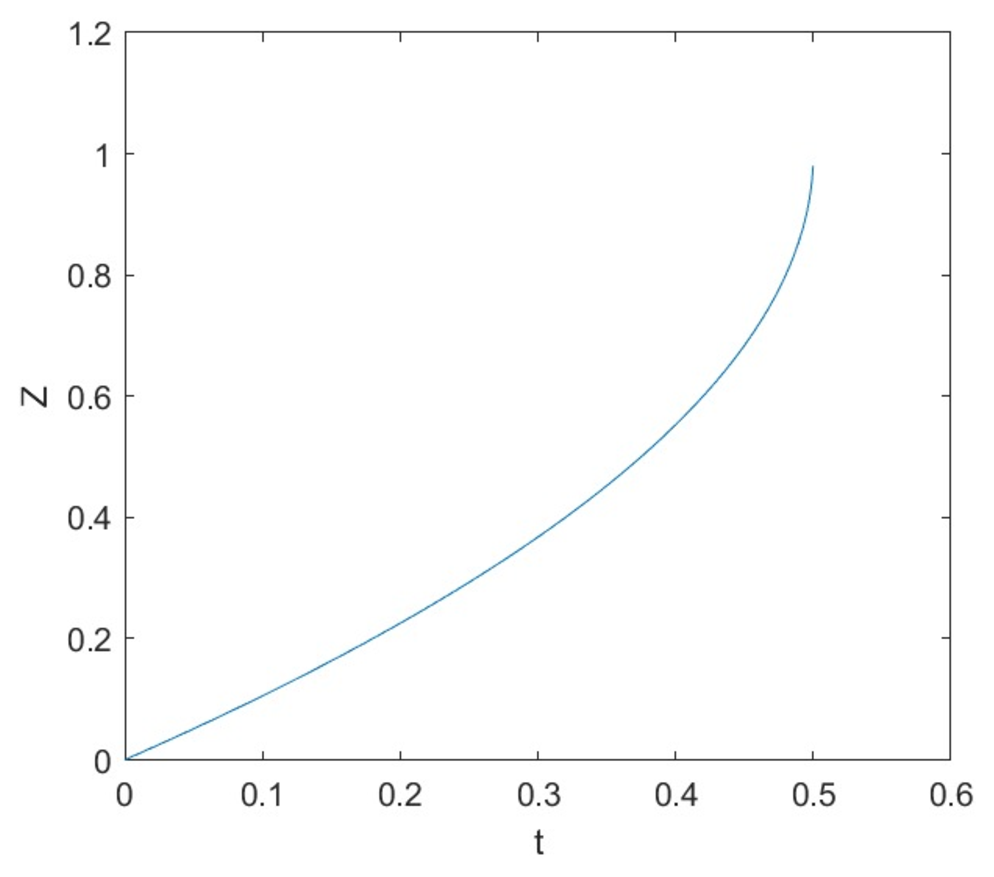
\includegraphics[width=0.8\textwidth]{Fig__36.eps}
\caption{This graphic shows the evolution over time of Z}
\end{figure}

\newpage
\section{Graphic user interface}
\begin{figure}[h]
\centering
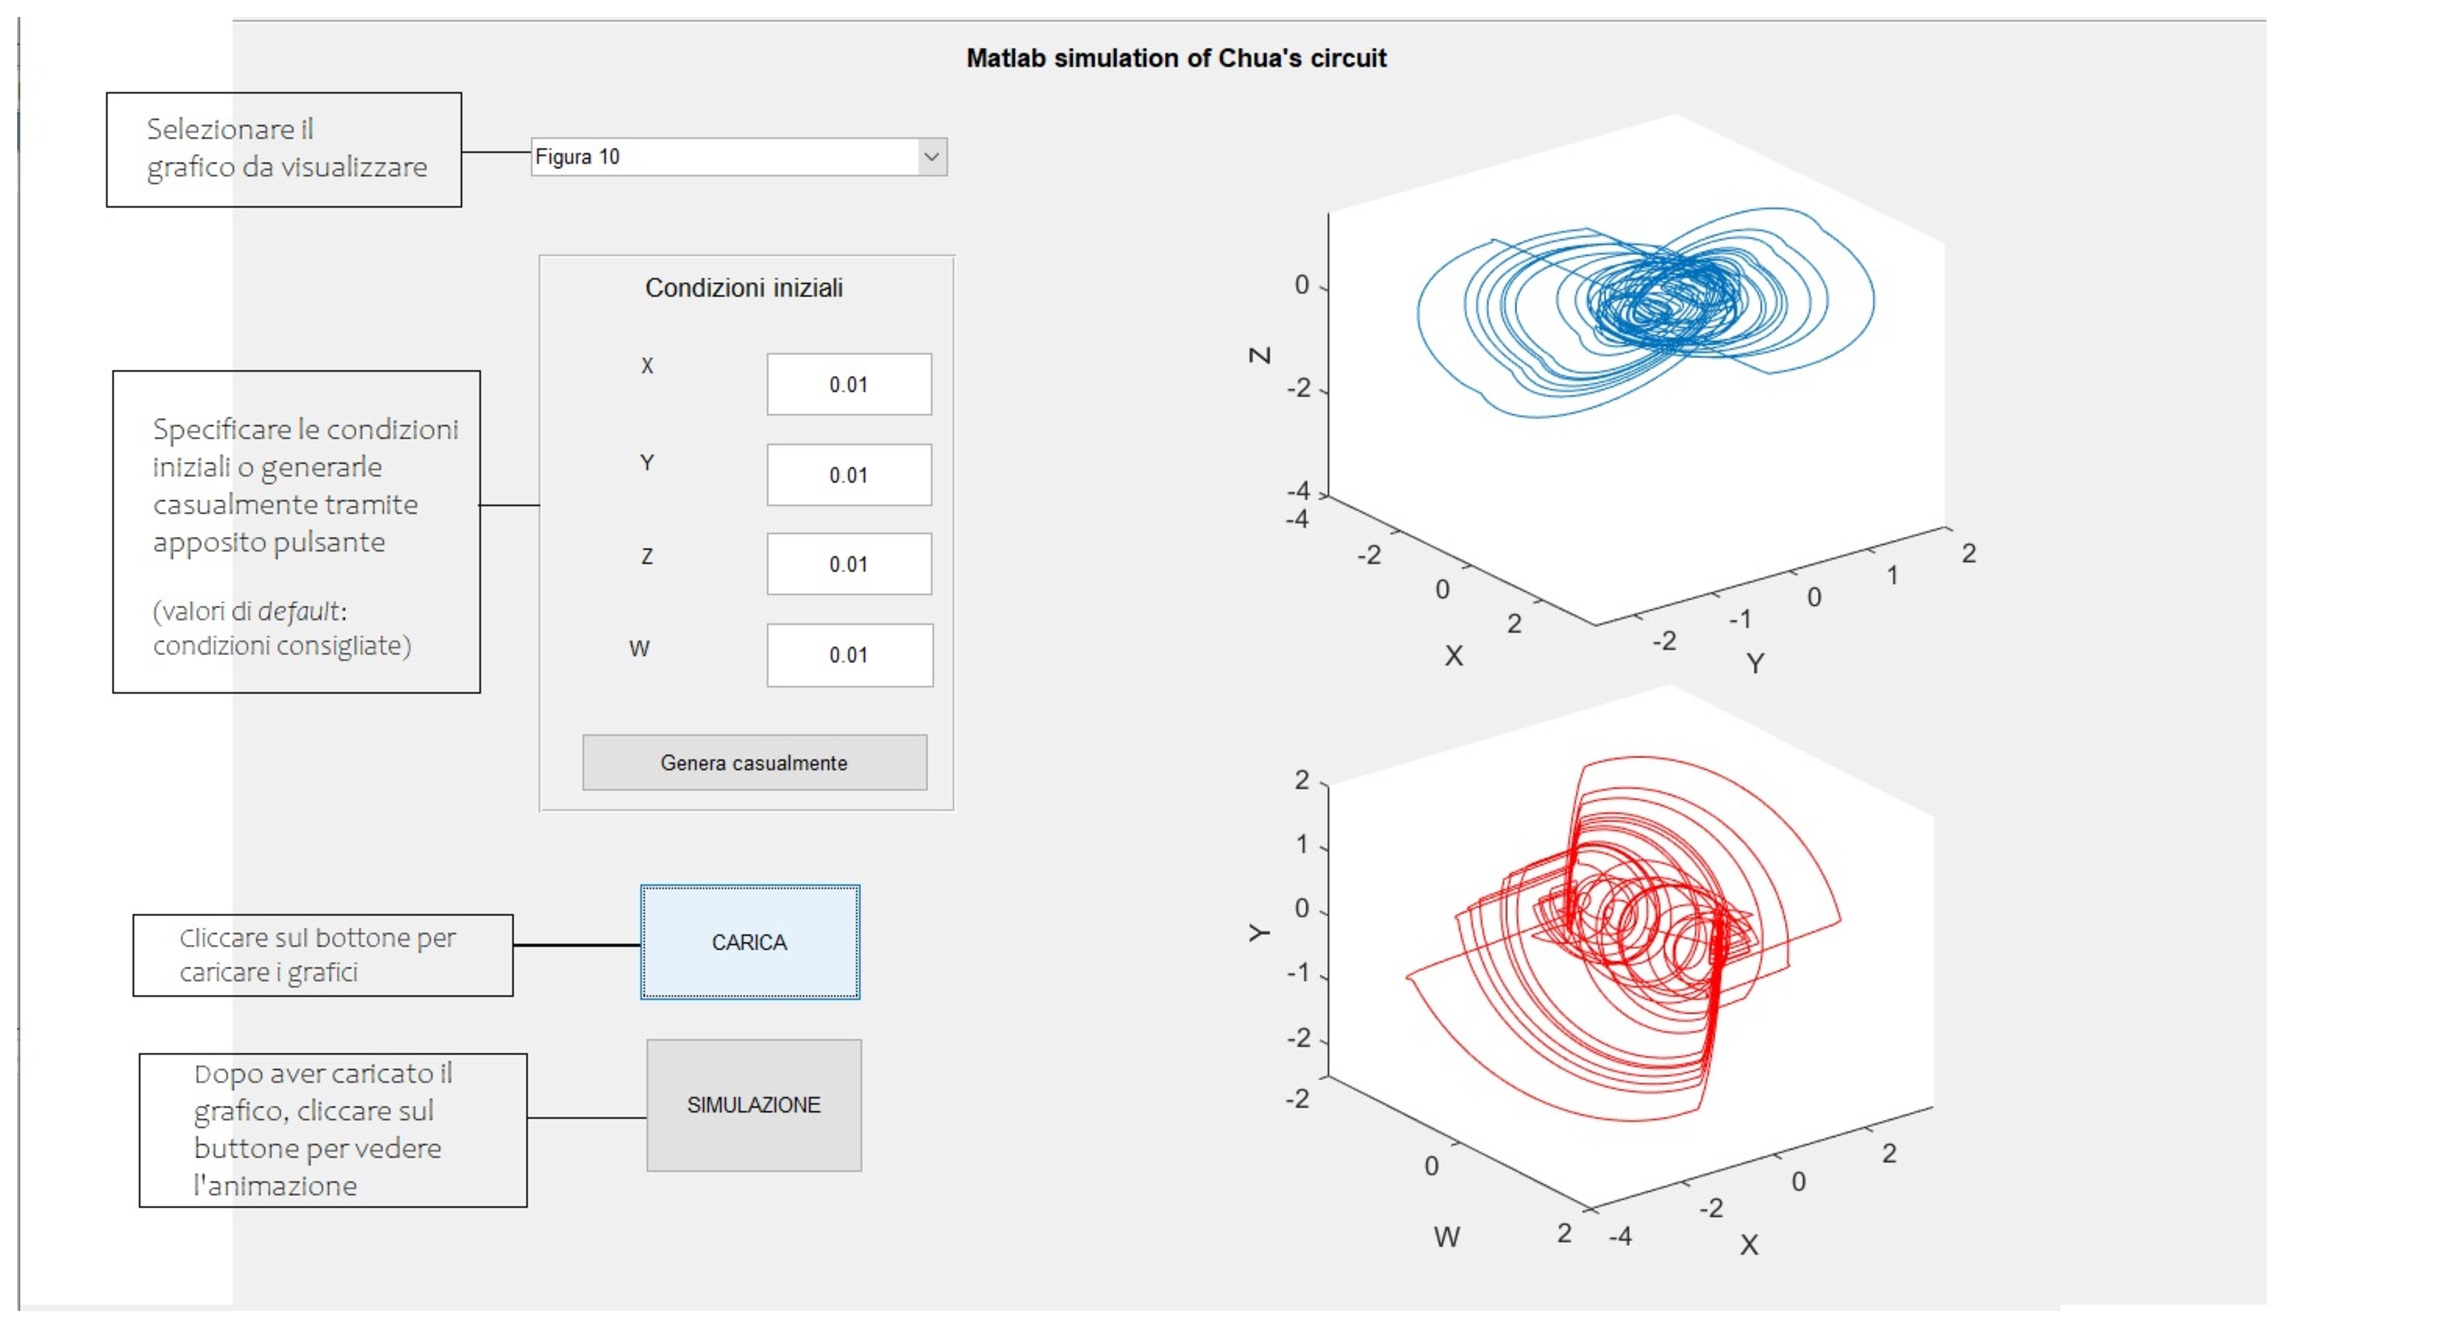
\includegraphics[width=1.3\textwidth]{gui_2.eps}
\end{figure}

\newpage
\section{Conclusion}
\subsection{Memristor}
After reading the article on oscillators, we  developed interest in the memristors themselves and did some research.  In particular, these two aspects struck us:

\subsubsection{How did HP develop its memristor?}
The HP component consists of a thin film of titanium dioxide sandwiched between two electrodes.
At the beginning there are two layers of film, one of which has a slight depletion of oxygen atoms. The oxygen vacancies act as charge carrier. The depleted film has a much lower resistance than the other. 
Under the effect of an electric field,  these gaps change, hence the resistance of the film depends on how much charge has previously circulated there.

\begin{figure}[h]
\centering
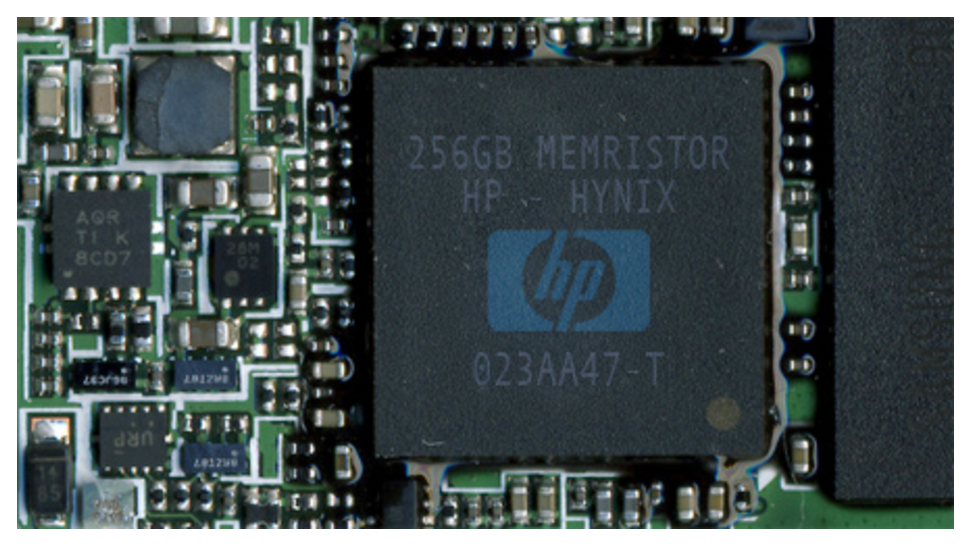
\includegraphics[width=0.8\textwidth]{Hp_memristor_1.eps}
\end{figure}

\subsubsection{PoliMi super computer}
Furthermore, we were intrigued by a recent research carried out by Polimi on this topic.
A PoliMi team led by Daniele Ielmini is building the fastest computer in the world, using memristors.
Their idea is to reduce the calculation time by carrying out the calculations directly in the memory
without, therefore, displacements of information.
To realize this idea they are using a grid of memristors, which allow to store analog values and complete calculations in memory.

\subsection{MatLab and LaTeX}
As students of computer engineering, this project was, for us, an opportunity to
experiment with new programming languages such as MatLab and LaTeX.
The biggest challenge for us was to translate the equations we read in the article into  MatLab functions, from which to derive graphs.
Having this task,  we chose to write this report in LaTeX, so as to obtain a 
more precise and “scientific" result.
They are both languages of great potential, with varied and diverse applications.
They will also be very useful, both for facing the the challenge of our next courses and in our future workplaces.

\subsection{Deepen old courses}
While working on the project we needed to retrace our steps to better understand
everything we read. For example,  we explored various aspects of Mathematical Analysis 2, working  mainly with differential equations.
We studied, in depth, methods for solving systems of differential equations, such as
that of Runge-Kutta of fourth and fifth order, noting, later, that it would also have been very useful
to have had knowledge of MatLab programming during the courses of  Mathematical Analysis or Geometry.

\subsection{Teamwork}
One of the best things was to work in a team.
Sometimes we splitted the tasks and worked in parallel, at other times,
we met and worked together to deal with the most difficult parts.
We had the opportunity to compare and share our ideas and develop a supportive atmosphere.

\subsection{Our Sincere Appreciation}
\textit{“Last, but not least"} we would like to thank Prof. Fiori for giving us the opportunity to work on this 
project and for being  constantly available to clarify our doubts.

\bibliographystyle{plain}
\bibliography{./bibliography}


\end{document}